\chapter{Deep Q-Network training maze resolution}
\section{Background}
The task was developed in python using available libraries for reinforcement learning such as Keras and Gym.
\begin{itemize}
    \item \textbf{Keras: }An open source library that provides an interface for artificial intelligence and neural networks tasks. It is based on the interface of TensorFlow library.
    \item \textbf{OpenAI Gym: }It is a toolkit for developing and comparing reinforcement learning algorithms. Gym library is a collection of environments, without assumptions about the agent, and support the reinforcement learning libraries (Tensorflow and Theano). The environments have a shared interface to help the developers to write algorithms and custom environments.
\end{itemize}

Deep Q Learning is suitable for this task because it is a typically problem framed as Markov Decision Process (a set of states S and actions A). The transitions are performed with probability P and reward R for a discounted gamma. 
The Q-Network proceeds as a non linear approximation which maps states in an action value. During the training, the agent interacts (fits) with the environment and the data received during the learning of the network.
The original article that start DQN can be found here https://www.cs.toronto.edu/~vmnih/docs/dqn.pdf.

The final goal is to approximate the non linear function \textit{Q(S,A)} with the deep learning of a multi layers neural network. The DQN, like for the supervised neural network, has loss function to predict the next state (assuming state s, action a and reward r).

\section{Implementation}
The source code is divided in two files \textit{main.py} and \textit{nnModel.py}.
In the first one are defined:
\begin{itemize}
    \item \textbf{Grid class: }Our custom environment, defined with gym interface for environments, which required to override specific methods: 
    \begin{itemize}
        \item \textit{init: }The class initializer requires the subset of \textit{walls states}, maximum dimension of the grid and the available steps for the agent (\textit{path\_length}). 
        The initializer defines attributes of the maze: action space, observation space, actual state, path lenth, target state and the walls susbset.
        \item \textit{step: }This function set the movement and the reward of the agent. It returns the state, reward, done (a boolean that check the status of the episode) and a log variable called info.
        \item \textit{render: }Visualization of the problem, not implemented for this task.
        \item \textit{reset: }At the end of the episode it resets actual state and path variables.
        \end{itemize}
    \item \textbf{model: }In this variable is stored the status of the neural network, e.g. it is possible check the architecture using\textit{ .summary()}. 
    \item \textbf{utilities: }Several functions are defined to plot, time logging, printing and saving weights of the network.

\end{itemize}

In the second file are implemented the deep neural network and the agent:
\begin{itemize}
    \item \textbf{build\_model: }Requires in input the dimension (or shape) of possible states and the number of actions. It is a deep sequential model, so each of the three layer is activated in sequence and the output layer has linear function that returns and array with the four probabilities of the 4 actions available.
    The structure is the following:
    \begin{enumerate}
        \item \textbf{Input layer: }It receives the states and actions and start to build with 64 neurons and an activation function "ReLU" that fires to the next layer.
        \item \textbf{Hidden layer: }It reduces the features space to 32 neurons and fires with ReLU activation function to the last layer
        \item \textbf{Output layer: }It reduce the actions space with a linear function to the actual agent's actions and returns the four probabilities.
    \end{enumerate}
    \item \textbf{build\_agent: }Requires in input the nn model and the number of actions. It returns a dqn agent with a policy (BoltzmannQPolicy), a memory state and the actual trained agent.
    
    \textit{BoltzmannQPolicy: }The action distribution is divided by actions parameters. The Boltzmann policy build a spectrum between picking the action randomly and the most optimal solution. In fact, the distribution gives the probability measure that a system will be in certain state of a function with parameters (in the original work are temperature and energy). 
    
    The agent \textit{dqn} is returned to the main process for the fitting with model and environment. 
\end{itemize}

\section{Experiments}

The environment is initialize calling \textit{Grid} class and passing the required parameters. 

For the training experiments we are considering a grid 64x64 with 11 obstacles and a path length of 500 steps. 

In the picture below are reported some results of the network training in 130 epochs. It is possible see the time interval for each epochs, between 0.5 second and 4 sec. The difference between the epochs it is to be brought to the machine time to do 500 steps and the achivement from the agent of the target state.

\begin{figure}[h]
    \centering
   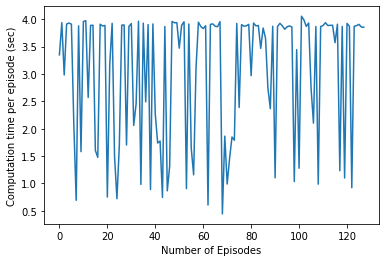
\includegraphics[width=\linewidth]{img/epochVStime}
    \caption{Time to resolution per epoch}
    \label{fig:my_label}
\end{figure}
The expected mean time distribution per episode is a monotonic descendent function. 
\begin{figure}[h]
    \centering
    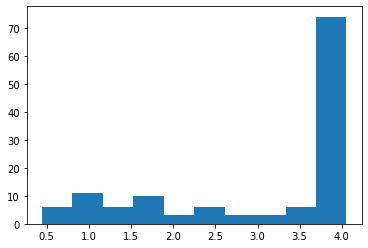
\includegraphics[width=\linewidth]{img/histTimeEps.png}
    \caption{Time distribution of the epochs}
    \label{fig:my_label}
\end{figure}
We are expecting an inversion of the following histogram, where the frequencies with high frequencies on short computational time and less number of longer runs will be exchange. 

